\documentclass[14pt]{article}

\usepackage[polish]{babel}
\usepackage[utf8]{inputenc}
\usepackage[T1]{fontenc}
\usepackage{extsizes}
\usepackage{graphicx}
\usepackage{tocloft}
\usepackage{amsmath}
\usepackage{multirow}
\usepackage{hyperref}


\font\titlefont=cmtt10 at 22pt

\title{
    
\includegraphics[scale=0.5]{images/logo-pwr-pion.png}
    \vspace{1cm}
    \\
    {\textbf{
    \titlefont Sygnały i obrazy cyfrowe
    \\ Laboratorium 4 - Poissoning
    }}
}
    
\author{
    Informatyczne Systemy Automatyki
    \\
    \\ Wykonujący:
    \\ Igor Potyrała - 272518
    \\
    \\ Prowadzący - Przemysław Śliwiński
}
\date{Data laboratoriów: 6 grudnia 2023}


\begin{document}
\maketitle
\newpage
% Spis treści
%\newpage
%\renewcommand{\cftsecleader}{\cftdotfill{\cftdotsep}}
%{
 % \hypersetup{linkcolor=black, hidelinks}
 % \tableofcontents
%}

% Wstęp teoretyczny, definicje
\section{Zadania}
\subsection{Cel zajęć}
Zadanie polega na porównaniu jakości 
interpolacji obrazów o niskim poziomie 
sygnału względem szumu z wykorzystaniem 
rozkładu Poissona.


\subsection{Wyniki}
\vspace{1cm}
\begin{center}
    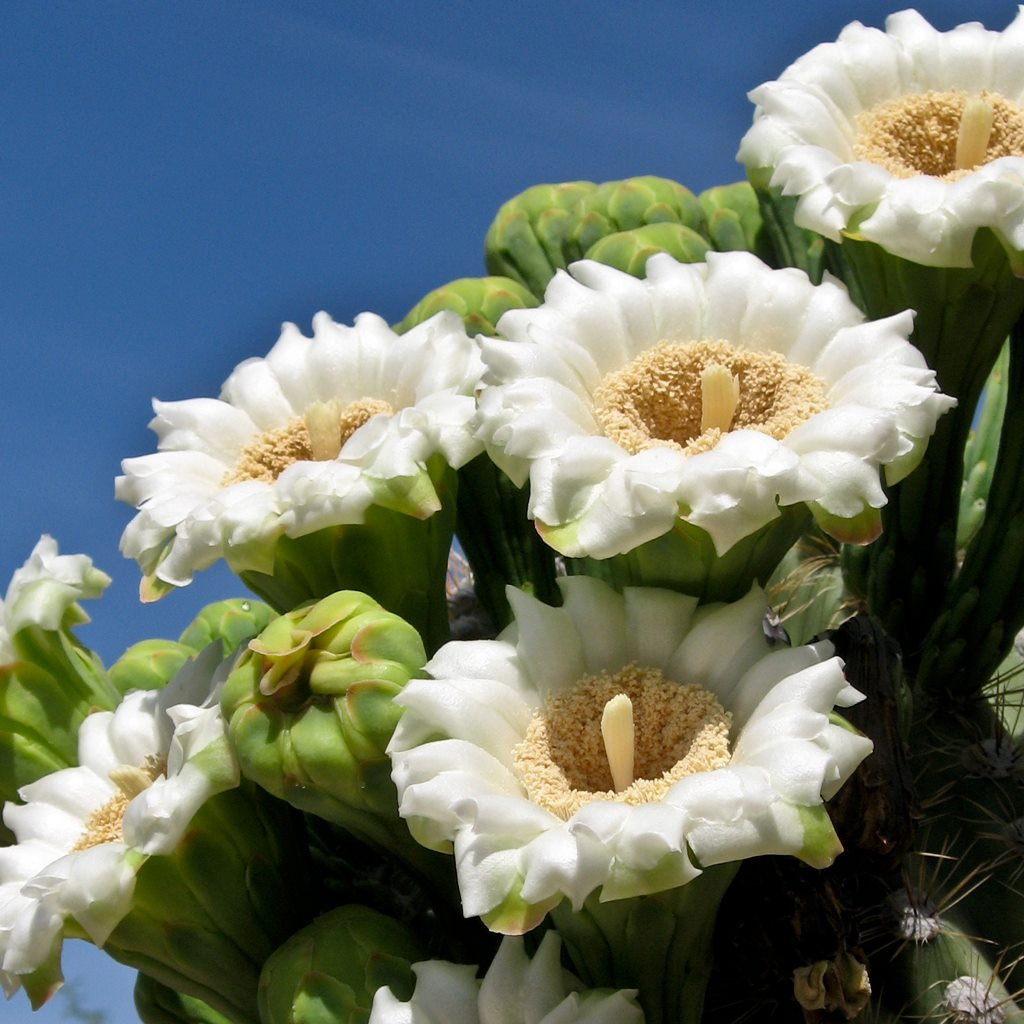
\includegraphics[scale=0.2]{images/cactus.jpg}
    \\ \small Obraz 1. Oryginalny obraz.

    % Lambda 4
    \vspace{0.5cm}
    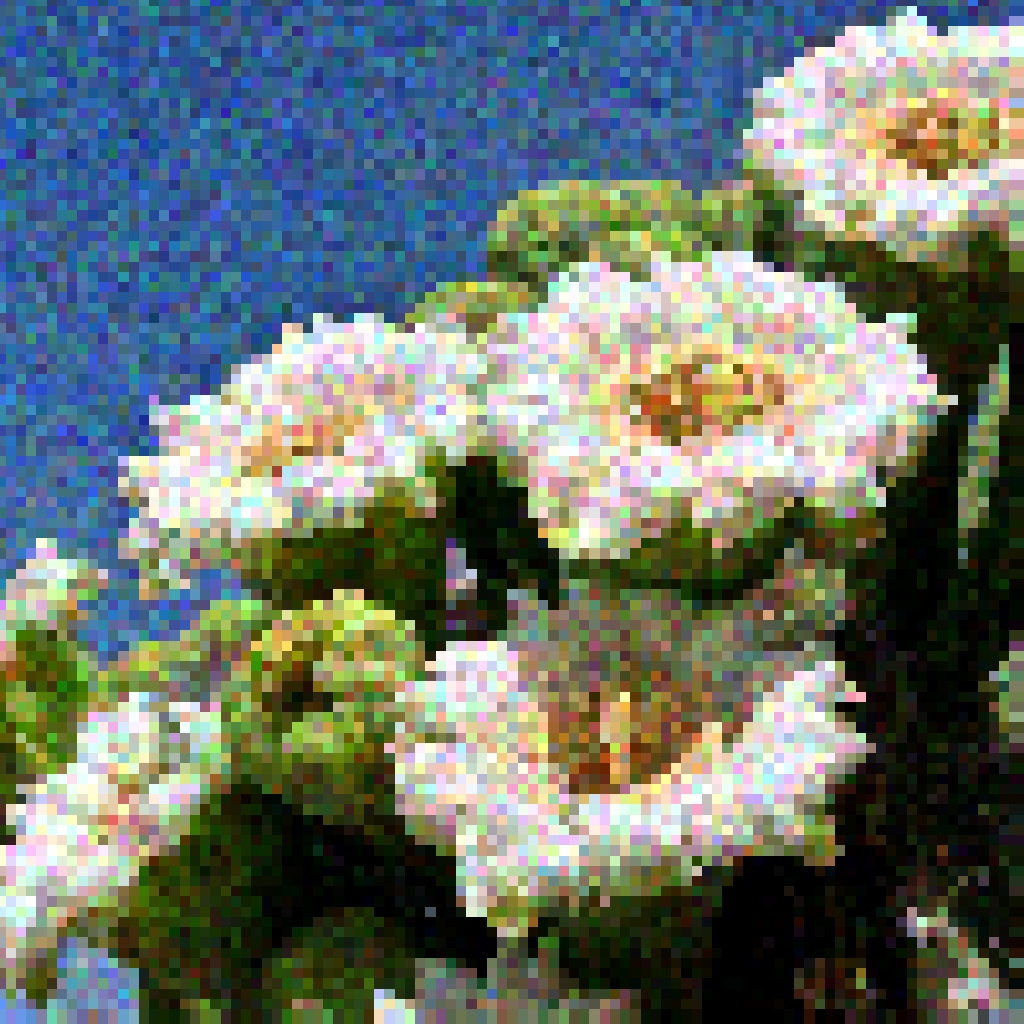
\includegraphics[scale=0.15]{images/Poisson_nearest_4x.jpg}
    \\ \small Obraz 2. po interpolacji najbliższego sąsiada, 
    $\lambda = 4$.

    \vspace{0.5cm}
    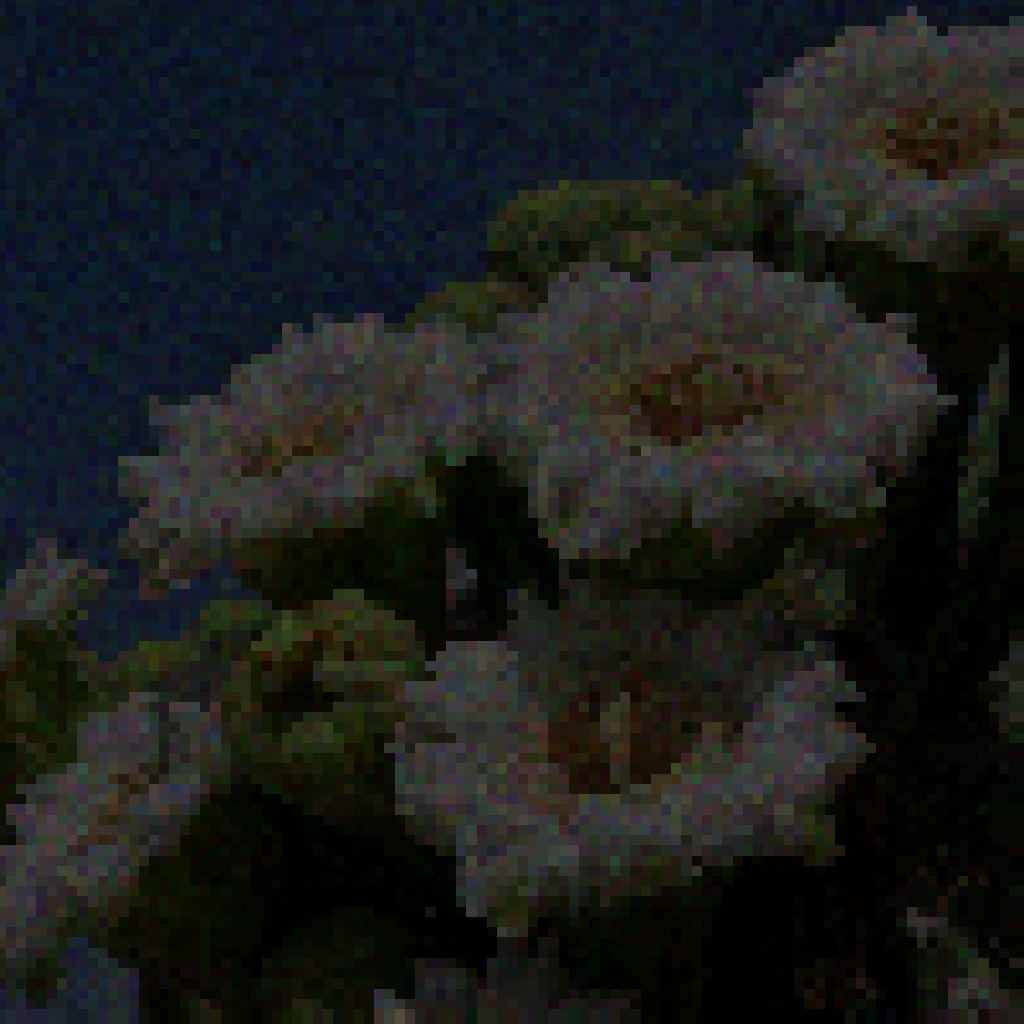
\includegraphics[scale=0.15]{images/Poisson_nearest_dark_4x.jpg}
    \\ \small Obraz 3. po interpolacji najbliższego sąsiada, 
    $\lambda = 4$, ciemny.

    % Lambda 4
    \vspace{0.5cm}
    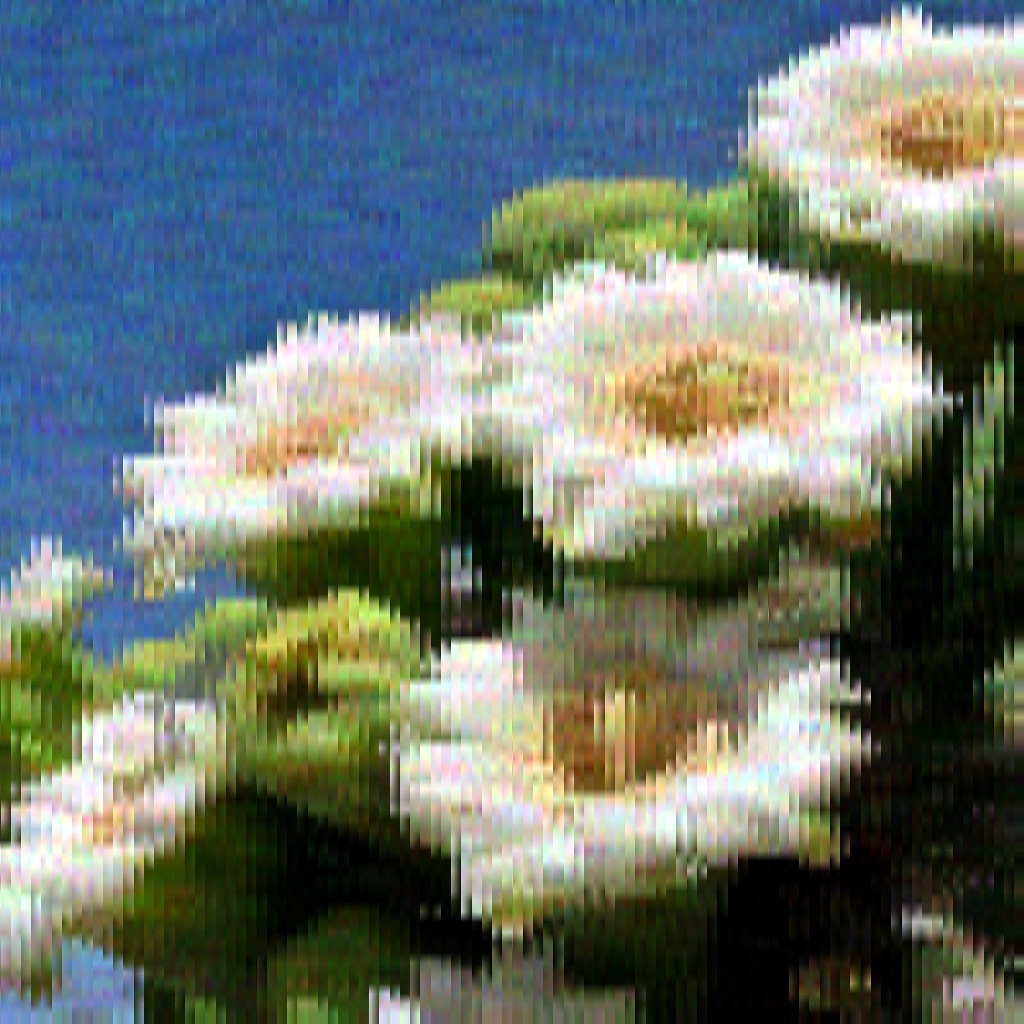
\includegraphics[scale=0.15]{images/Poisson_bilinear_4x.jpg}
    \\ \small Obraz 4. po interpolacji linearnej, 
    $\lambda = 4$.

    \vspace{0.5cm}
    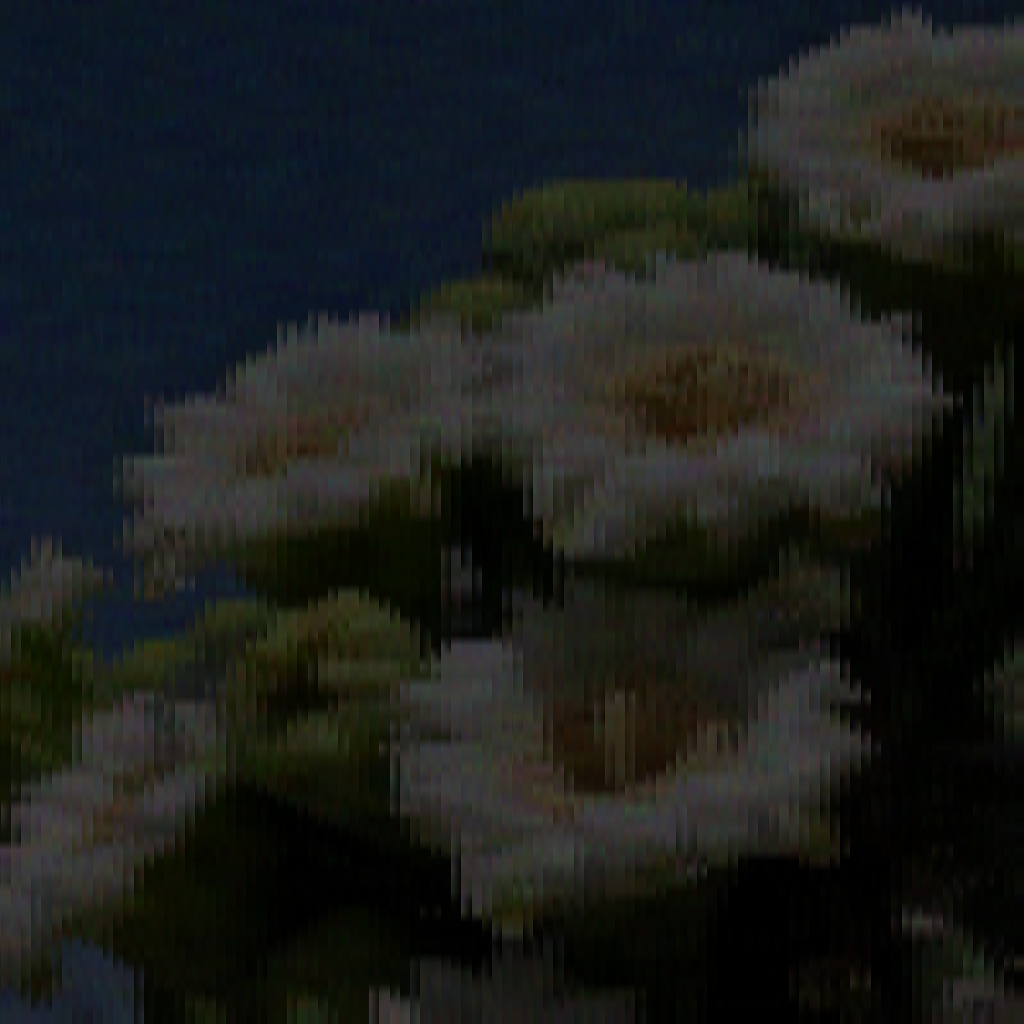
\includegraphics[scale=0.15]{images/Poisson_bilinear_dark_4x.jpg}
    \\ \small Obraz 5. po interpolacji linearnej, 
    $\lambda = 4$, ciemny.

    % Lambda 4
    \vspace{0.5cm}
    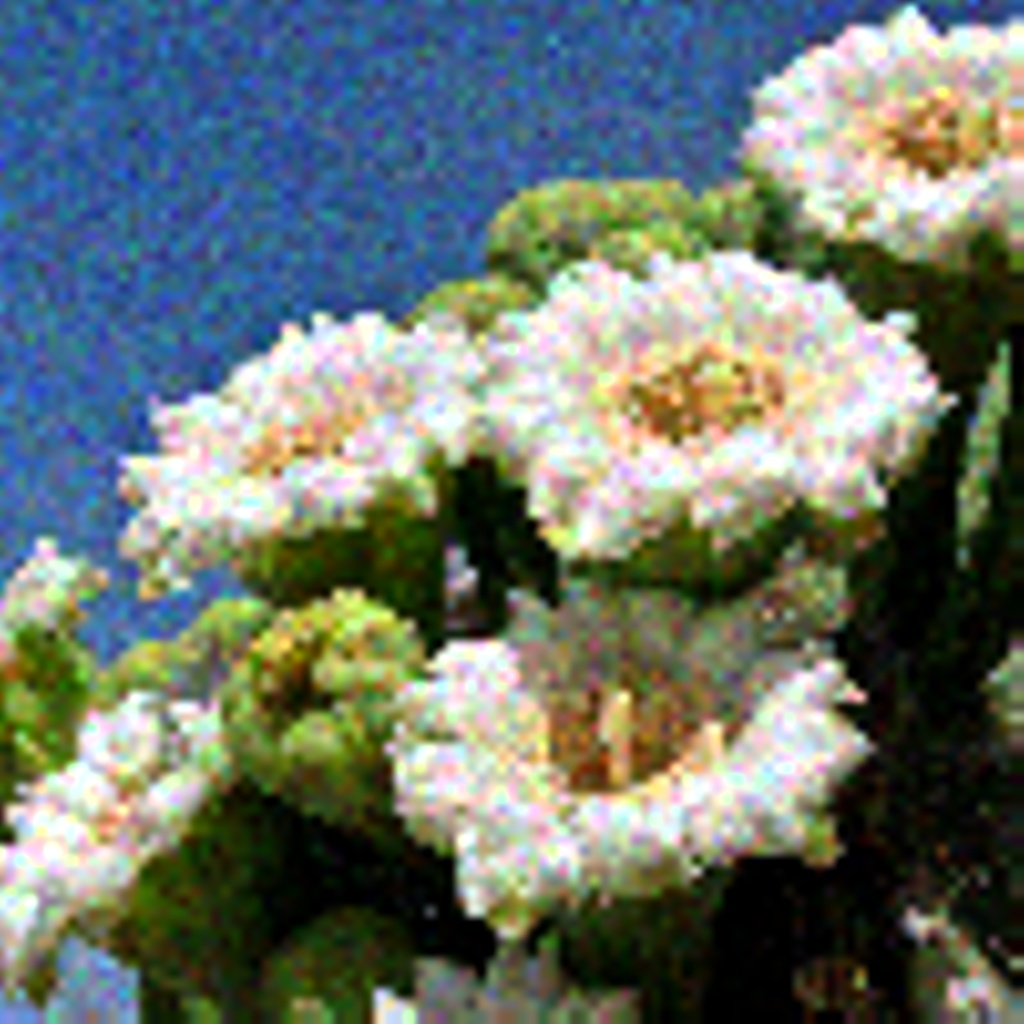
\includegraphics[scale=0.15]{images/Poisson_keys_4x.jpg}
    \\ \small Obraz 6. po interpolacji funkcją Keysa, 
    $\lambda = 4$.

    \vspace{0.5cm}
    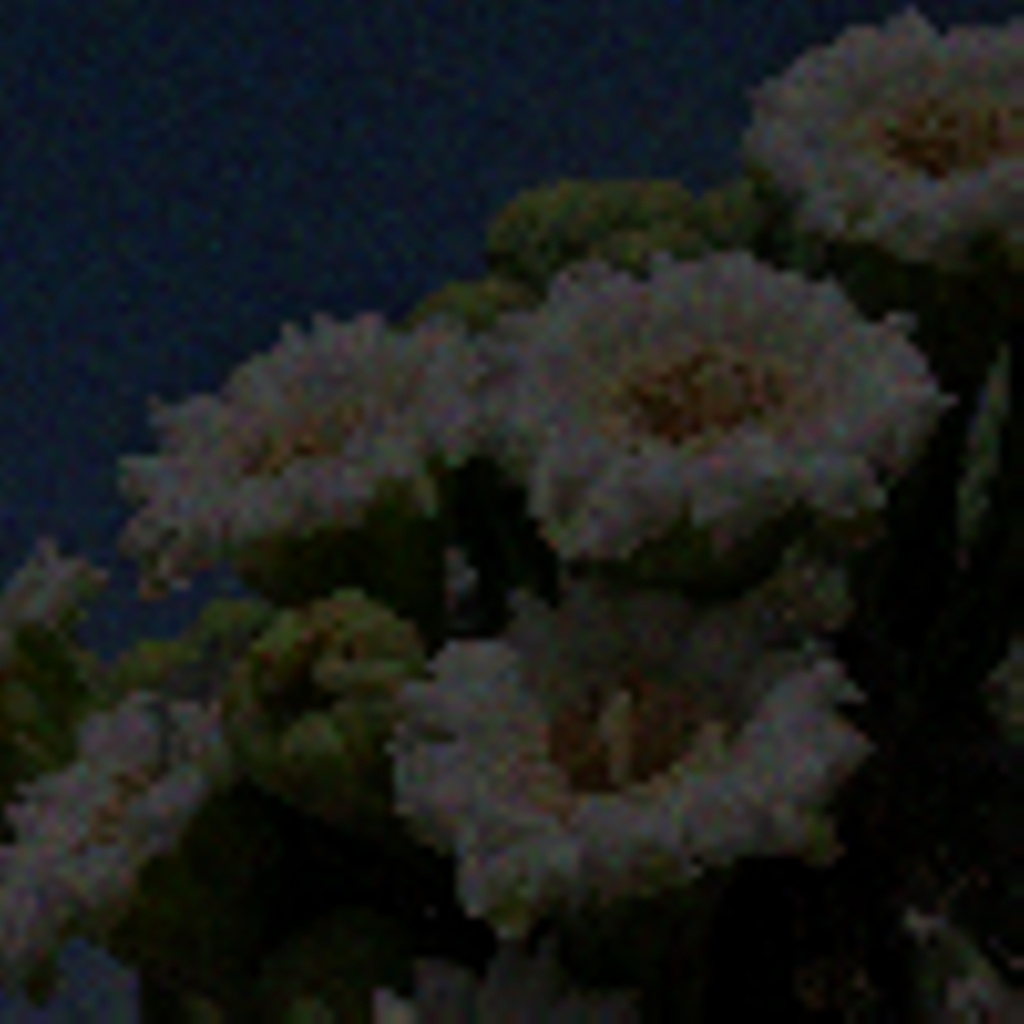
\includegraphics[scale=0.15]{images/Poisson_keys_dark_4x.jpg}
    \\ \small Obraz 7. po interpolacji funkcją Keysa, 
    $\lambda = 4$, ciemny.

    %%%%%%%%%%%%%%%%%%%%%%%%%%%%%%%%%%%%%%%%%%%%%%%
    % Lambda 16
    \vspace{0.5cm}
    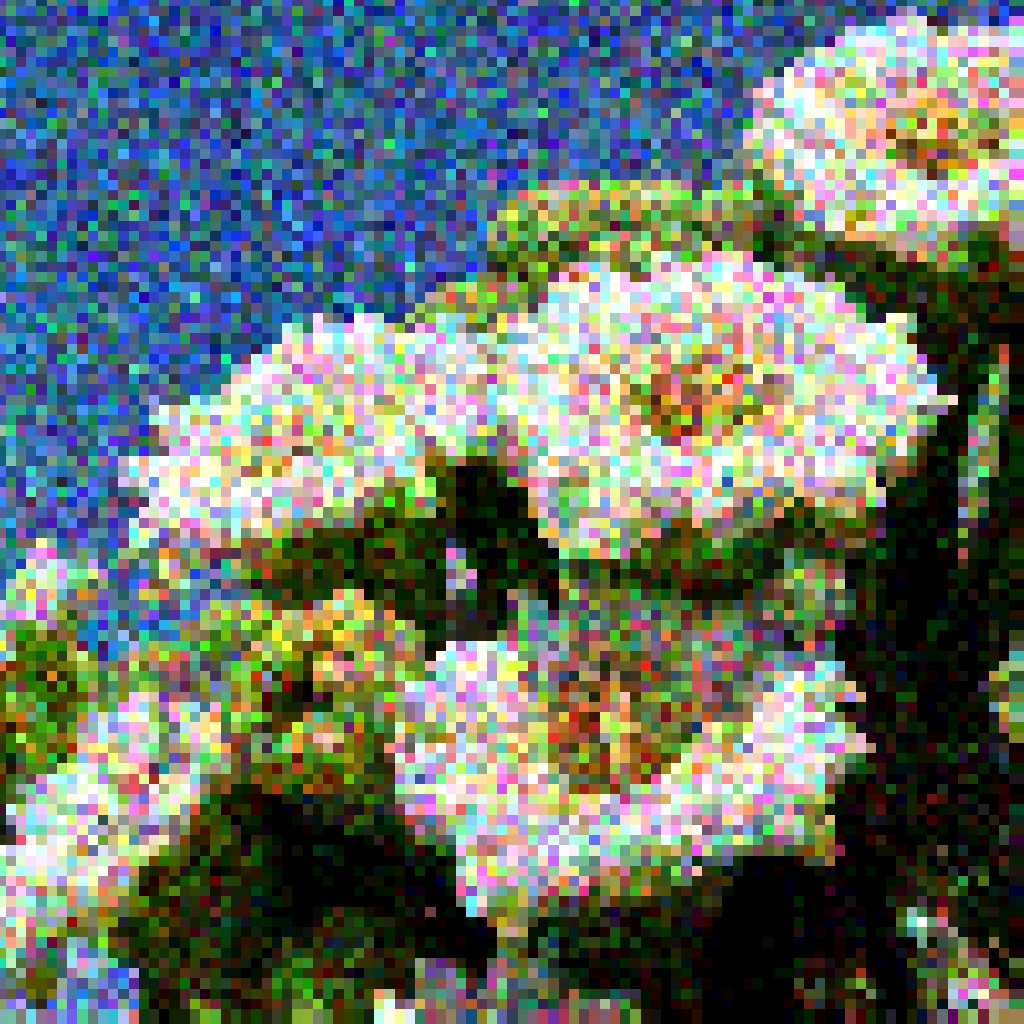
\includegraphics[scale=0.15]{images/Poisson_nearest_16x.jpg}
    \\ \small Obraz 8. po interpolacji najbliższego sąsiada, 
    $\lambda = 16$.

    \vspace{0.5cm}
    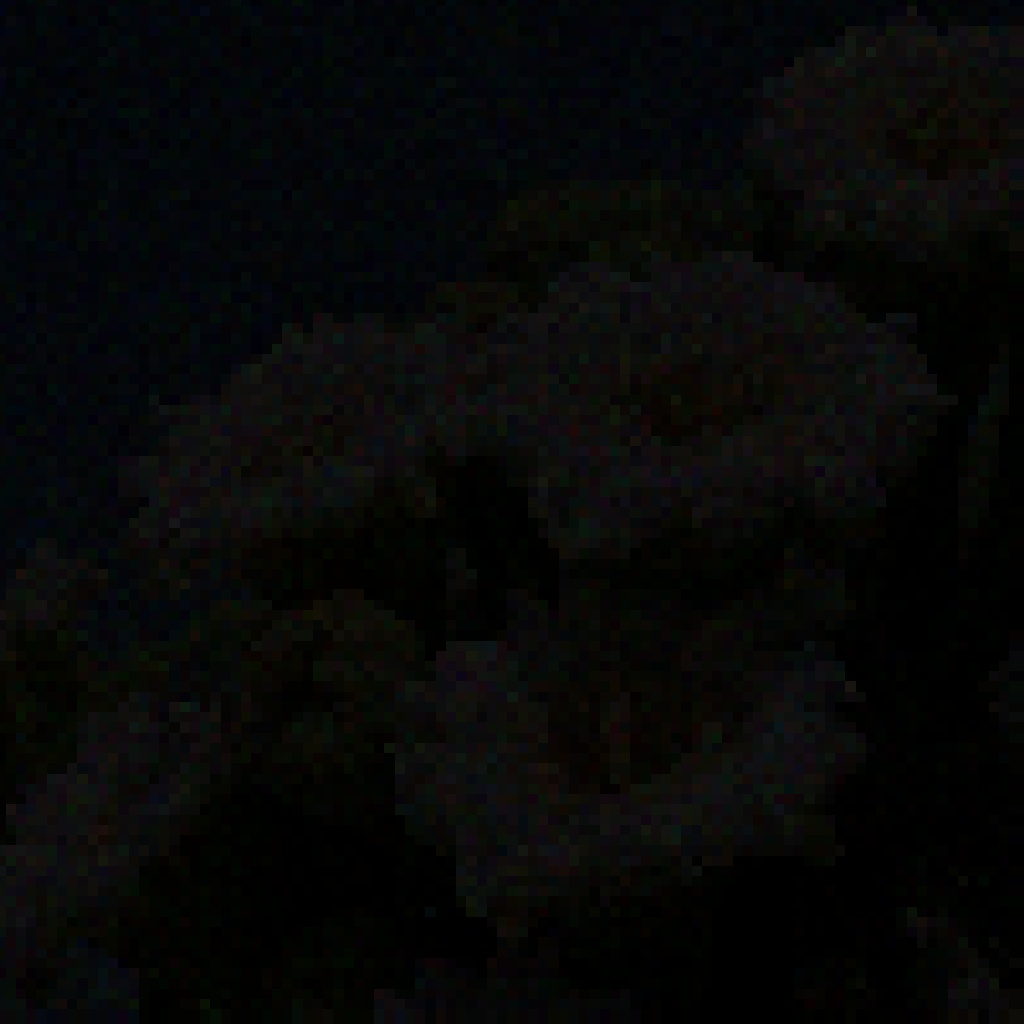
\includegraphics[scale=0.15]{images/Poisson_nearest_dark_16x.jpg}
    \\ \small Obraz 9. po interpolacji najbliższego sąsiada, 
    $\lambda = 16$, ciemny.

    \vspace{0.5cm}
    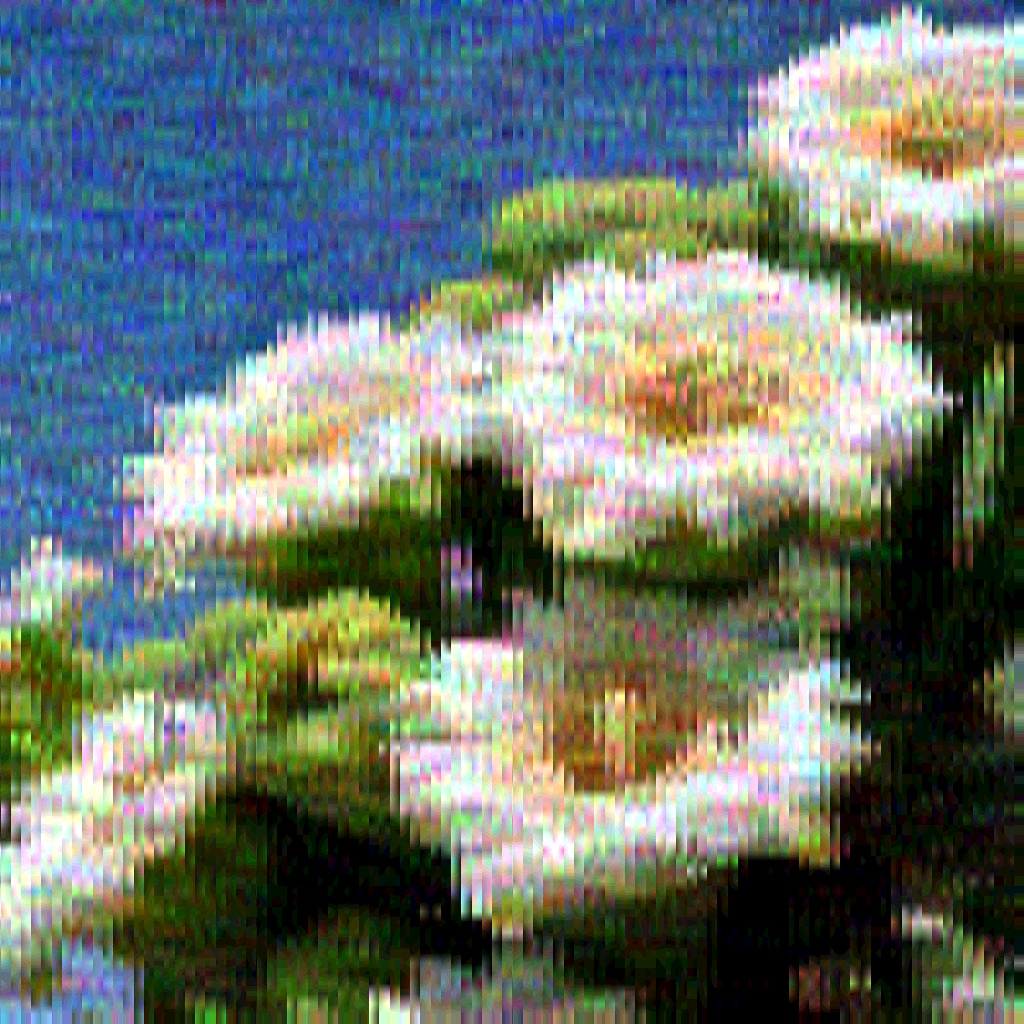
\includegraphics[scale=0.15]{images/Poisson_bilinear_16x.jpg}
    \\ \small Obraz 10. po interpolacji linearnej, 
    $\lambda = 16$.

    \vspace{0.5cm}
    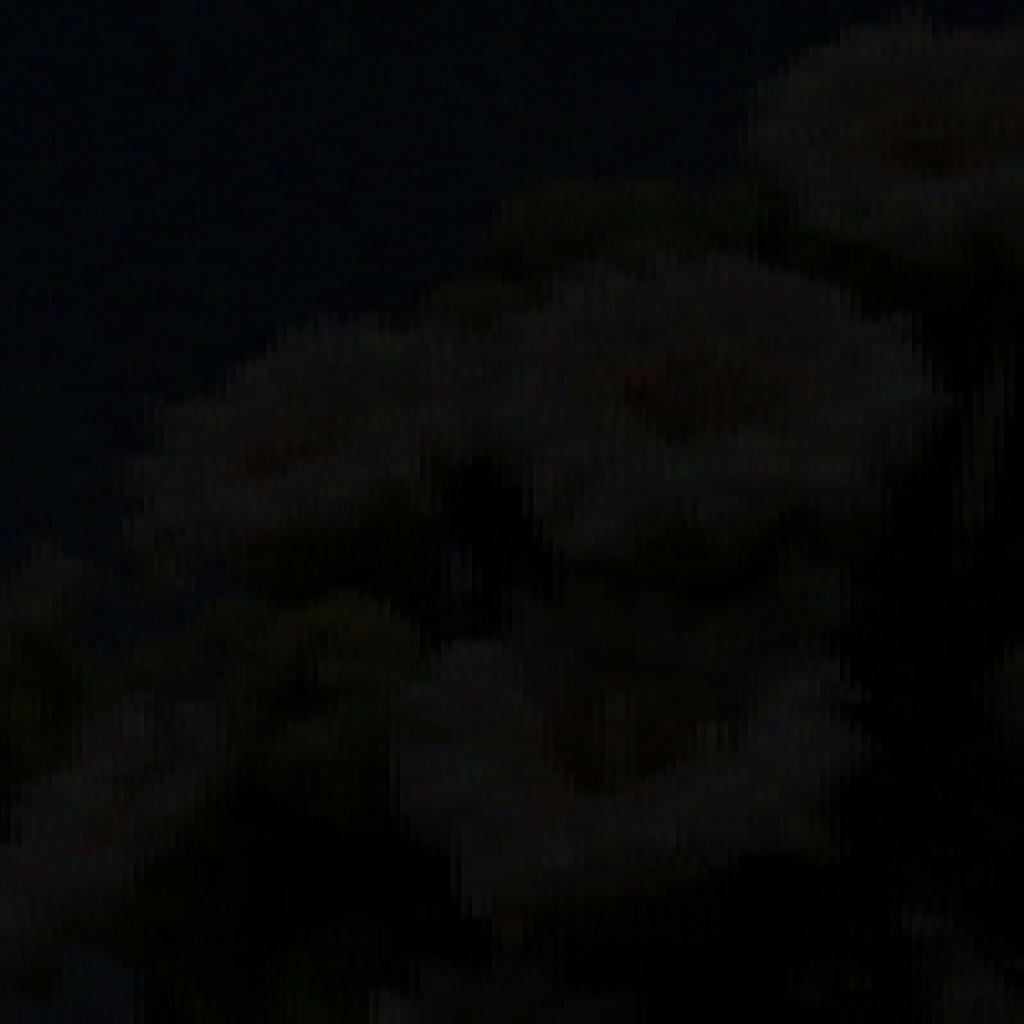
\includegraphics[scale=0.15]{images/Poisson_bilinear_dark_16x.jpg}
    \\ \small Obraz 11. po interpolacji linearnej, 
    $\lambda = 16$, ciemny.

    % Lambda 16
    \vspace{0.5cm}
    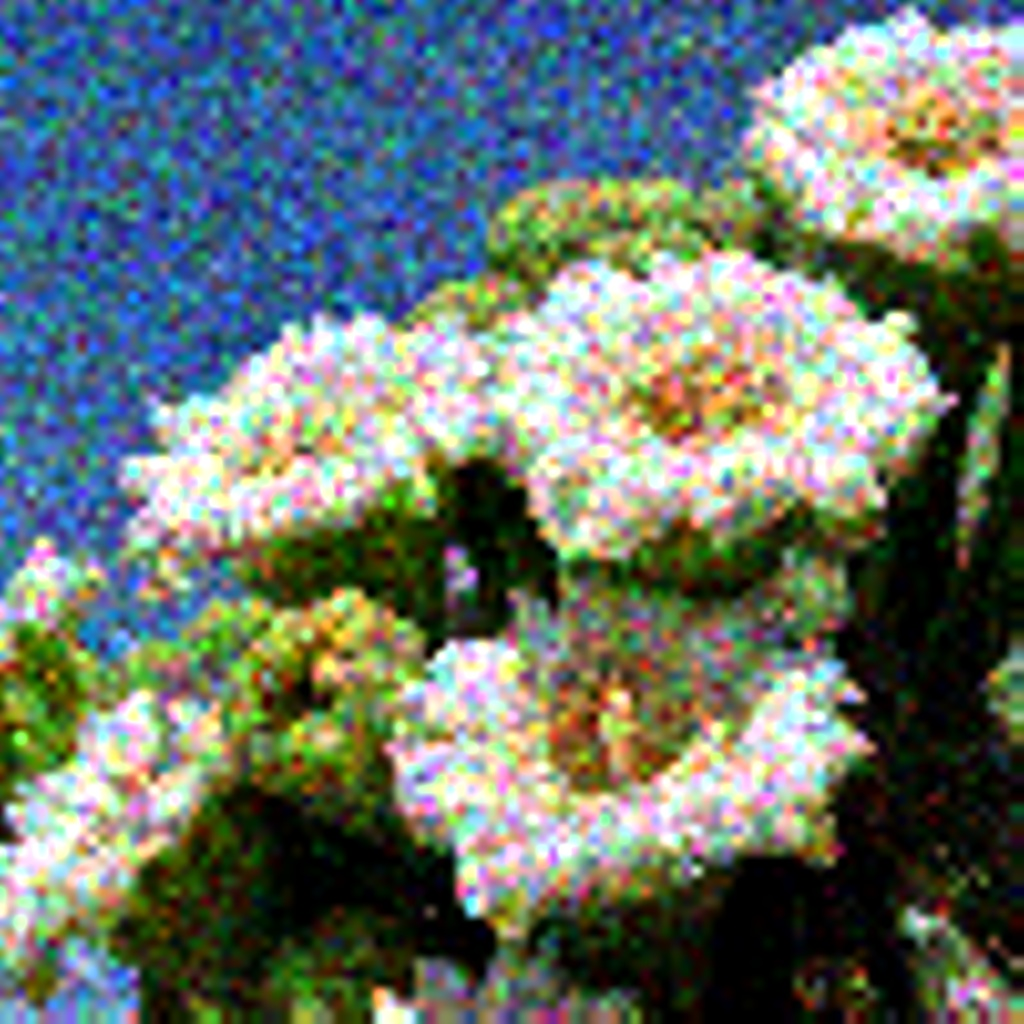
\includegraphics[scale=0.15]{images/Poisson_keys_16x.jpg}
    \\ \small Obraz 12. po interpolacji funkcją Keysa, 
    $\lambda = 16$.

    \vspace{0.5cm}
    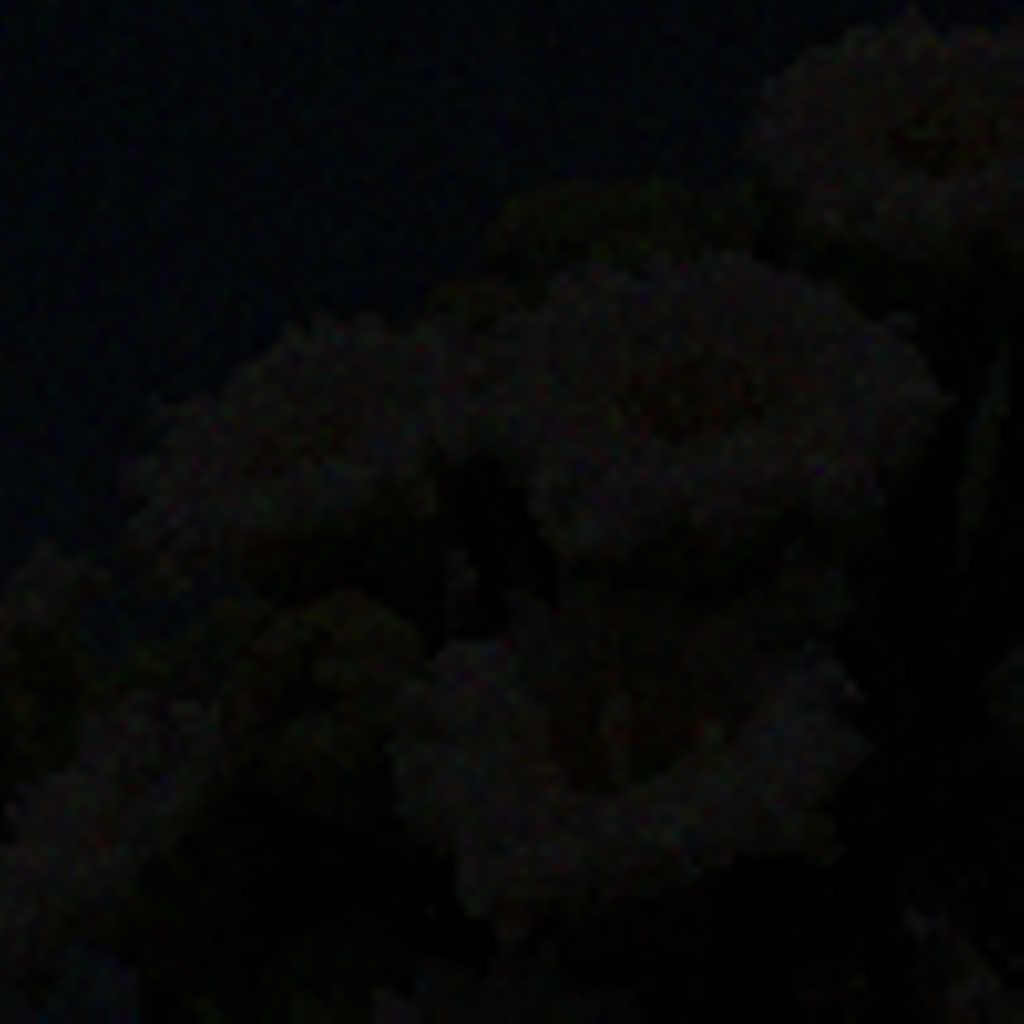
\includegraphics[scale=0.15]{images/Poisson_keys_dark_16x.jpg}
    \\ \small Obraz 13. po interpolacji funkcją Keysa, 
    $\lambda = 16$, ciemny.

    \vspace{1.5cm}
\end{center}

\newpage
\section{Wnioski}


\begin{center}
    Jedną z rzeczy, którą można zauważyć jest rozpikselowanie przy każdej
    z inerpolacji, a w przypadku interpolacji linearnej, także sporego rozmazania.

    \vspace{0.2cm}
    Obiektywnie patrząc, najlepiej w 
    obu przypadkach wypadła interpolacja liniowa, dla $\lambda=4$ 
    funkcja Keysa wypadła tylko odrobinę lepiej mając nieco mniejsze 
    błędy MSE oraz MAE, ale wadą w przypadku użycia interpolacji linearnej
    jest spore rozmazanie końcowego obrazu. Można także zauwayżyć zależność
    MSE oraz MAE od $\lambda$ (średnia liczba zarejstrowanych fotonów)
    - widać, że skala obu błędów powiększa się.


    \vspace{0.25cm}
    \begin{tabular}{|c|c|c|c|c|}
        % MSE - kwadratowy
        % MAE - absolutny
        \hline
        & \multicolumn{2}{|c|}{$\lambda = 4$} & \multicolumn{2}{|c|}{$\lambda = 16$}\\ \hline
        & MSE & MAE & MSE & MAE \\ \hline
        Naj. sąsiada & 837,98 & 19,68 & 2158,48 & 33,52 \\ \hline
        Linearna & 558,09 & 14,59 & 861,99 & 20,24 \\ \hline
        Keysa & 422,33 & 14,06 & 1002,45 & 22,84 \\ \hline

    \end{tabular}
    \vspace{0.2cm}
    \\ \small Tabela 1. przedstawiająca błędy MSE oraz MAE dla $\lambda=4$ i $\lambda=16$.
\end{center}

\end{document}